\documentclass[11pt]{article}
\usepackage[english]{babel}
\usepackage{enumitem}
\usepackage{fancyhdr}
\usepackage{amsfonts, amssymb}
\usepackage{graphicx}
\usepackage{caption}
%\usepackage[cm]{fullpage} %%formats everything to maximize space (can edit easily use wiki)
\usepackage{amsmath}   
\usepackage{avant}
\usepackage{graphicx}
\usepackage{amsthm}  %Theorem Stuff
 \usepackage{algpseudocode}
 \usepackage{tikz}
 \usepackage{url}
\usepackage[colorlinks, linkcolor=cyan, citecolor = cyan]{hyperref} %for table of contents
\usepackage[all]{hypcap}
\usepackage{sectsty} 
\usepackage[font = small, labelfont = bf, textfont= it, labelformat = empty]{caption}
\usepackage[labelformat = empty]{subcaption}
\usepackage{array}
\usepackage[landscape]{geometry}



\begin{document}
\begin{figure}\centering
 \begin{subfigure}[t]{0.3\textwidth}\centering

\includegraphics[width = 2in]{0.pdf}
\caption{Initial Configuration of Criminal Network.}\end{subfigure}
\quad
 \begin{subfigure}[t]{0.3\textwidth}\centering

\includegraphics[width = 2in]{1.pdf}
\caption{Officer chooses street criminal at random.}\end{subfigure}
\quad
 \begin{subfigure}[t]{0.3\textwidth}\centering
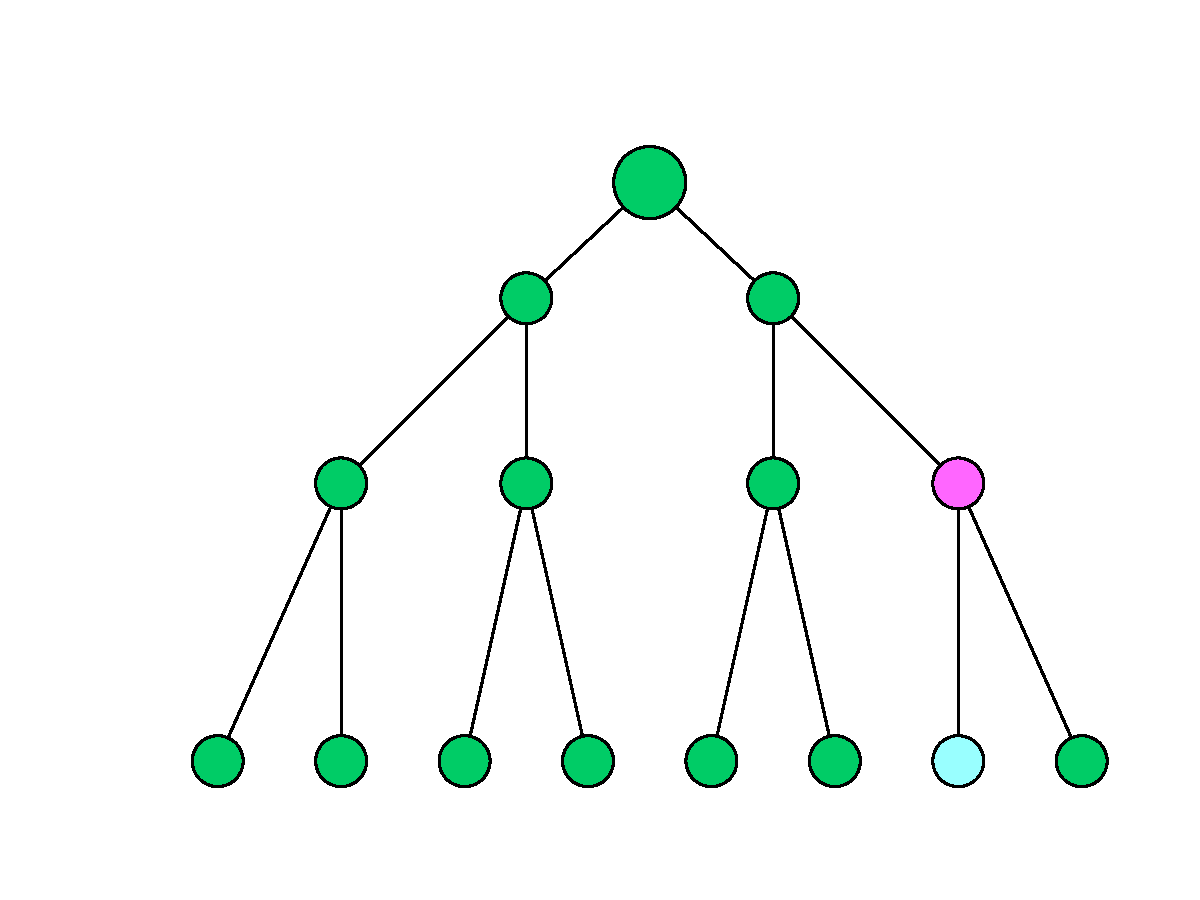
\includegraphics[width = 2in]{2.pdf}
\caption{Officer investigates the only neighbor of the street criminal.}\end{subfigure}
 \begin{subfigure}[t]{0.3\textwidth}\centering

\includegraphics[width = 2in]{3.pdf}
\caption{Officer arrests current criminal and his sub-syndicate.}\end{subfigure}
\quad
 \begin{subfigure}[t]{0.3\textwidth}\centering
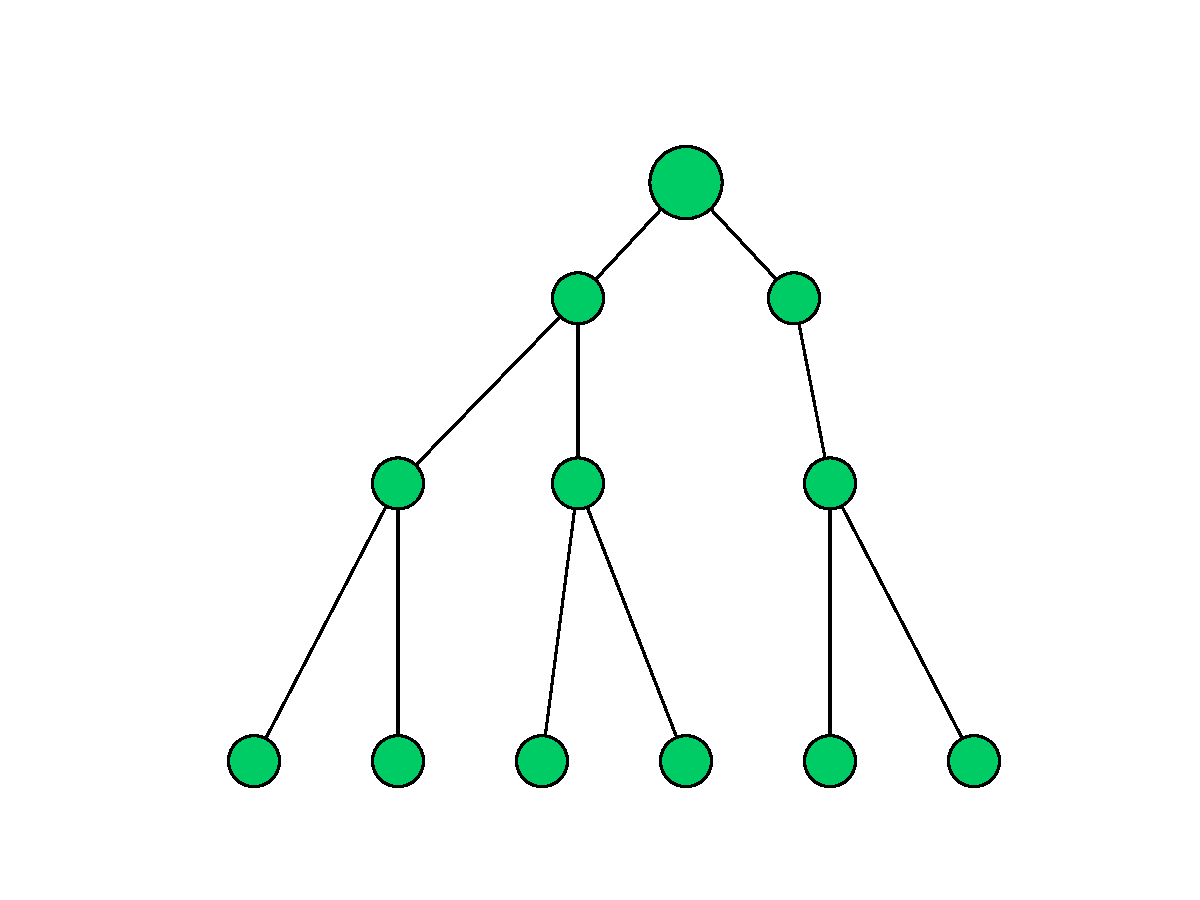
\includegraphics[width = 2in]{4.pdf}
\caption{Arrested nodes are removed from tree.}\end{subfigure}
\quad
 \begin{subfigure}[t]{0.3\textwidth}\centering
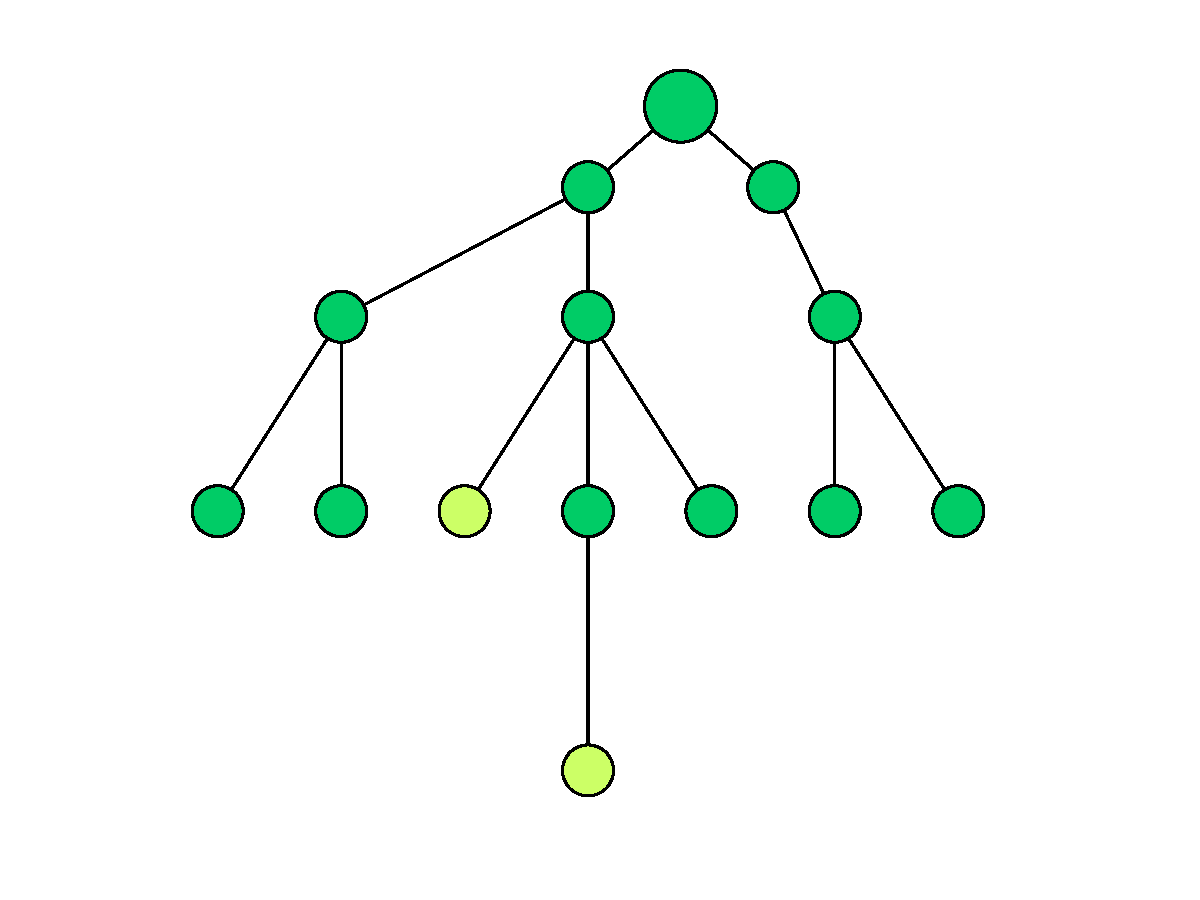
\includegraphics[width = 2in]{5.pdf}
\caption{Network undergoes preferential attachment growth.}\end{subfigure}
\hspace{1in}
\caption{}
\end{figure}

\end{document}